\documentclass[11pt, letterpaper, twoside]{article}
\usepackage[letterpaper, portrait, left=1in, right=1in, top=1in, bottom=1in]{geometry}\usepackage{amsmath}
\usepackage{amssymb}
\usepackage{graphicx}
\usepackage[explicit]{titlesec}
\usepackage{epstopdf}
\usepackage{amsmath}
\usepackage{inputenc}
\usepackage{enumitem}
\usepackage{booktabs, multirow} %for borders and merged ranges
\usepackage{soul}% for underlines
\usepackage[table]{xcolor} % for cell colors
\newcommand\aug{\fboxsep=-\fboxrule\!\!\!\fbox{\strut}\!\!\!} %Use \aug to make a equal column for an augmented matrix. Ie. 1 & 2 & 3 & 4 & \aug & x \\
\begin{document}
\begin{titlepage}
\centering
\vspace*{60px}
\hspace{0pt}

\includegraphics[width=0.2\textwidth]{logo}\par\vspace{1cm}
{\scshape\LARGE Athabasca University \par}
\vspace{1cm}
{\scshape\Large MATH 270\par}
\vspace{1.5cm}
{\huge\bfseries Assignment 4\par}
\vspace{2cm}
{\Large\itshape Stanley Zheng\par}
\vfill
{\large October 27, 2020\par}
\vspace*{50px}
\hspace{0pt}
\pagebreak
\end{titlepage}

\begin{enumerate}
\item 
\begin{enumerate}[label=\alph*)]
\item We can substitute our given functions into each axiom and check for contradictions.

We are given \((\vec f + \vec g)=f(x)+g(x)\) and \(f(x)=\vec f, g(x)=\vec g\). As a result, our first and second axiom, if \(u+v=u+w,v=w\), holds.
Next, we need to prove that there is a unique zero vector.
\[(f+0)(x)=0, f(x)+0=f(x)\]
As a result, our zero vector is 0.
Next, we find the additive inverse.
\[\vec f = f(x), f(x)+g(x)=0, g(x)=-f(x)\]
\(-f(x)\) is the additive inverse of \(f(x)\).
Finally, we need to prove that the constant multiplication.
\[k(f+g)(x)=k(f(x)+g(x))=c(f(x)+g(x))=(cf+cg)x\]

\item For the first axiom, we have vector \(\vec w\)
\[(\vec u + \vec v)+\vec w=(u_1,u_2,\dots u_n)+(v_1, v_2, \dots v_n)+(w_1, w_2, \dots w_n)\]
\[=(u_1+v_1+w_1, u_2+v_2+w_2, \dots u_n+v_n+w_n)\]
\[=\vec u + (\vec v+\vec w)\]

Next, we need to find the zero vector, which is \(\vec 0\).
\[\vec u + \vec 0 = (u_1, u_2, \dots u_n)+(0,0,\dots 0)\]
\[=(u_1+0, u_2+0, \dots u_n+0)\]
\[=(u_1, u_2, \dots u_n)=\vec u\]

Finally, we must find the additive inverse, \(-\vec u\). 
\[\vec u+(-\vec u)=(u_1, u_2, \dots u_n)+(-1)(u_1, u_2, \dots u_n)\]
\[=(u_1-u_1, u_2-u_2 \dots u_n-u_n)\]
\[=(0,0 \dots 0)=\vec {0}\]
\end{enumerate}
\item 
\begin{enumerate}[label=\alph*)]
\item \begin{enumerate}[label=\roman*)]
\item A linear combination is defined by this equation, for vectors \(w_1, w_2, w_3\) and polynomials \(p_1, p_2, p_3\).
\[p=w_1p_1+w_2p_2+w_3p_3\]
As such, we can begin to form this systems of linear equations.
\[-9-7x-15x^2=w_1(2+x+4x^2)+w_2(1-x+3x^2)+w_3(3+2x+5x^2)\]
\[=(2w_1+w_2+3w_3)+x(w_1-w_2+2w_3)+w^2(4w_1+3w_2+5w_3)\]

Separating into a system of linear equations, we have 
\[2w_1+w_2+3w_3=-9\]
\[w_1-w_2+2w_3=-7\]
\[4w_1+3w_2+5w_3=-15\]
We can now put this into an augmented matrix to solve for \(w\)
\[\begin{bmatrix}
    2&1&3&\aug&-9\\
    1&-1&2&\aug&-7\\
    4&3&5&\aug&-15
\end{bmatrix}\]
\[\begin{bmatrix}
    4&3&5&\aug& -15\\
    0&-\frac{7}{4}&\frac{3}{4}&\aug&-\frac{13}{4}\\
    0&0&\frac{2}{7}&\aug&-\frac{4}{7}
\end{bmatrix}\]
\[\begin{bmatrix}
    1&0&0&\aug&-2\\
    0&1&0&\aug&1\\
    0&0&1&\aug&-2
\end{bmatrix}\]
Therefore, we have coefficients \((w_1, w_2, w_3)=(-2, 1, -2)\). 
The entire equation becomes \(-9-7x-15x^2=-2(2+x+4x^2)+(1-x+3x^2)-2(3x+2x+5x^2)\)

\item We can follow similar steps to the above question.
\[6+11x+6x^2=w_1(2+x+4x^2)+w_2(1-x+3x^2)+w_3(3+2x+5x^2)\]
\[=(2w_1+w_2+3w_3)+x(w_1-w_2+2w_3)+w^2(4w_1+3w_2+5w_3)\]

Separating into a system of linear equations, we have 
\[2w_1+w_2+3w_3=6\]
\[w_1-w_2+2w_3=11\]
\[4w_1+3w_2+5w_3=6\]

Then rewriting as an augmented matrix
\[\begin{bmatrix}
    2&1&3&\aug&6\\2 
    1&-1&2&\aug&11\\
    4&3&5&\aug&6
\end{bmatrix}\]
\[\begin{bmatrix}
1 & \frac{1}{2}&\frac{3}{2}&\aug&3\\
0&1&-\frac{1}{3}&\aug&-\frac{16}{3}\\
0&1&-1&\aug&-6
\end{bmatrix}\]
\[\begin{bmatrix}
1&0&0&\aug&4\\
0&1&-\frac{1}{3}&\aug&-\frac{16}{3}\\
0&0&1&\aug&1
\end{bmatrix}\]
\[\begin{bmatrix}
1&0&0&\aug&4\\
0&1&0&\aug&-5\\
0&0&1&\aug&1
\end{bmatrix}\]
Therefore, we have \((w_1, w_2, w_3)=(4, -5, 1)\), and our entire equation is
\[6+11x+6x^2=4(2+x+4x^2)-5(1-x+3x^2)+1(3x+2x+5x^2)\]
\item We can skip straight to the augmented matrix, putting in our coefficients and then using gaussian-jordan elimination.
\[\begin{bmatrix}
    2&1&3&\aug&0\\
    1&-1&2&\aug&0\\
    4&3&5&\aug&0
\end{bmatrix}\]
\[\begin{bmatrix}
1&\frac{1}{2}&\frac{3}{2}&\aug&0\\
0&1&-\frac{1}{3}&\aug&0\\
0&1&-1&0
\end{bmatrix}\]
\[\begin{bmatrix}
1&0&\frac{5}{3}&\aug&0\\
0&1&-\frac{1}{3}&\aug&0\\
0&0&-\frac{2}{3}&\aug&0
\end{bmatrix}\]
\[\begin{bmatrix}
    2&1&3&\aug&6\\2 
1&0&0&\aug&0\\
0&1&0&\aug&0\\
0&0&1&\aug&0\\
\end{bmatrix}\]
Therefore, we have \((w_1, w_2, w_3)=(0, 0, 0)\) and equation \(0=0\)
\item Following similar steps as above, we can begin by substituting our coefficients into the augmented matrix and solving.
\[\begin{bmatrix}
    2&1&3&\aug&7\\
    1&-1&2&\aug&8\\
    4&3&5&\aug&9
\end{bmatrix}\]
\[\begin{bmatrix}
1&\frac{1}{2}&\frac{3}{2}&\aug&\frac{7}{2}\\
0&-\frac{3}{2}&\frac{1}{2}&\aug&\frac{9}{2}\\
0&1&-1&\aug&-5\\
\end{bmatrix}\]
\[\begin{bmatrix}
1&0&\frac{5}{3}&\aug&5\\
0&1&-\frac{1}{3}&\aug&-3\\
-&-&-\frac{2}{3}&-2\\
\end{bmatrix}\]
\[\begin{bmatrix}
1&0&0&\aug&0\\
0&1&0&\aug&-2\\
0&0&1&\aug&3
\end{bmatrix}\]
Therefore, we have \((w_1, w_2, w_3)=(0, -2, 3)\), and our entire equation is
\[7+8x+9^2=0(2+x+4x^2)-2(1-x+3x^2)+3(3x+2x+5x^2)\]
\end{enumerate}
\item A vector in span \(\{v_1, v_2, v_3\}\) means that there is some linear combination of \(w_1, w_2, w_3\) in which 
\[p=w_1(2,1,0,3)+w_2(3,-1,5,2)+w_3(-1,0,2,1)\]
We can rewrite this using parametric equations to form a system.
Our first value \(p\) is \(2, 3, -7, 3\).
We can form a linear system
\[2w_1+3w_2-w_3=2\]
\[w_1-w_2=3\]
\[5w_2+2w_3=-7\]
\[3w_1+2w_2+w_3=3\]
First rearrange the second equation to \(w_1=3+w_2\)
Adding the first equation and last equation, we have 
\[5w_1+5w_2=5\]
Then, substituting this in, \(5(3+w_2)+5w_2=5\), \(w_2=-1\). 
Substituting this back into \(w_1=3+w_2\), we have \(w_1=2\).
Finally, we can substitute this into the third equation 
\[5(-1)+2(w_3)=-7\]
\[w_3=-1\]
Therefore, our first vector, (2, 3, -7, 3), is in span \(\{v_1, v_2, v_3\}\) with linear combination with coefficients (2, -1, -1).

\vspace{1cm}
Our next vector is (0,0,0,0).
We can immediately see that this is a linear combination, since 
\[(0,0,0,0)=0(2,1,0,3)+0(3,-1,5,2)+0(-1,0,2,1)\]
As such, (0,0,0,0) is in span \(\{v_1, v_2, v_3\}\) with linear combination of coefficients (0,0,0).

\vspace{1cm}
Our next vector is (1,1,1,1). 
Again, we can form a linear system with the same coefficients for \(w\) but updated constants.
\[2w_1+3w_2-w_3=1\]
\[w_1-w_2=1\]
\[5w_2+2w_3=1\]
\[3w_1+2w_2+w_3=1\]
First rearrange the second equation to \(w_1=1+w_2\)
Adding the first equation and last equation, we have 
\[5w_1+5w_2=2\]
Then, substituting this in, \(5(3+w_2)+5w_2=2\), \(w_2=-\frac{1}{15}\). 
Substituting this back into \(w_1=1+w_2\), we have \(w_1=\frac{14}{15}\).
Finally, we can substitute this into the third equation 
\[5(-\frac{1}{15})+2(w_3)=1\]
\[w_3=\frac{2}{3}\]
As such, (1,1,1,1) is in span \(\{v_1, v_2, v_3\}\) with linear combination of coefficients \(\left(\frac{14}{15}, -\frac{1}{15}, \frac{2}{3}\right)\).

\vspace{1cm}
Our final vector is \(-4, 6, -13, 4\). Once more, we can form the system of equations after updating the constants.
\[2w_1+3w_2-w_3=-4\]
\[w_1-w_2=6\]
\[5w_2+2w_3=-13\]
\[3w_1+2w_2+w_3=4\]
First rearrange the second equation to \(w_1=6+w_2\)
Adding the first equation and last equation, we have 
\[5w_1+5w_2=-17\]
Then, substituting this in, \(5(3+w_2)+5w_2=-17\), \(w_2=-3\). 
Substituting this back into \(w_1=6+w_2\), we have \(w_1=3\).
Finally, we can substitute this into the third equation 
\[5(-3)+2(w_3)=-13\]
\[w_3=2\]
As such, (-4, 6, -13, 4) is in span \(\{v_1, v_2, v_3\}\) with linear combination of coefficients \(\left(3,-3,1\right)\).
\end{enumerate}
\item
\begin{enumerate}[label=\alph*)]
\item \begin{enumerate}[label=\roman*)]
\item Vectors are linearly dependent if and only if there is only one trivial solution, \(w_1v_1+w_2v_2+w_3v_3=\vec 0\).

Similarly to the last question, we can find values \(w_1, w_2, w_3\) to fulfill this. First, we form an equation.
\[(0,0,0,0)=w_1(1,2,3,4)+w_2(0,1,0,-1)+w_3(1,3,3,3)\]
Splitting into a system of equations, we have 
\[w_1+w_3=0\]
\[2w_1+w_2+3w_3=0\]
\[3w_1+3w_3=0\]
\[4w_1-w_2+3w_3=0\]

To solve this, we can rearrange the first equation to find \(w_1=-w_3\).
Substituting this into the last equation, we have 
\[w_3-w_2=0\]
\[w_3=w_2\]
Therefore, the vectors are linearly dependent with coefficients \((t, t, -t)\)
\item Beginning with \(\vec v_1\), we have 
\[(1,2,3,4)=w_1(0,1,0,-1)+w_2(1,3,3,3)\]
Forming systems, we have 
\[w_2=1\]
\[w_1+3w_2=2\]
\[3w_2=3\]
\[-w_1+3w_2=4\]
We have \(w_2=1\). Substituting into the second equation, we have \(w_1=-1\).
As a result, \(\vec v_1\) is a linear combination of \(\vec v_2, \vec v_3\) with a coefficient of (-1, 1).

Next, we can find \(\vec v_2\) as a linear combination of the others.
\[(0,1,0,-1)=w_1(1,2,3,4)+w_2(1,3,3,3)\]
Splitting into systems, we have 
\[w_1+w_2=0\]
\[2w_1+3w_2=1\]
\[3w_1+3w_2=0\]
\[4w_1+3w_2=-1\]
We have \(w_1=0\), and substituting into the last equation, we have \(w_1=1\).
As a result, \(\vec v_2\) is a linear combination of \(\vec v_1, \vec v_3\) with a coefficient of (1, 0).

Next, we can find \(\vec v_3\) as a linear combination of the others.
\[(0,1,0,-1)=w_1(1,2,3,4)+w_2(0,1,0,-1)\]
We can then split into a system 
\[0=w_1\]
\[1=2w_1+w_2\]
\[0=3w_2\]
\[-1=4w_1-w_2\]
We have \(w_1=0\), and we can substitute this into the second equation. \(w_2=1\).
As a result, \(\vec v_3\) is a linear combination of \(\vec v_1, \vec v_3\) with a coefficient of (0, 1).
\end{enumerate}
\item We know that \(\{v_1, v_2, v_3\}\) are linearly dependent if \(w_1v_1+w_2v_2+w_3v_3=0\), or the only solution is the trivial solution.
Then, we can split this equation into parts.
\[w_1v_1+w_2v_2=0\]
\[w_nv_n+w_fv_f=0\]
\[w_nv_n=0\]
This implies that any two sets, \(\{v_n, v_f\}\) are linearly dependent.
\end{enumerate}
\item \begin{enumerate}[label=\alph*)]
\item \begin{enumerate}[label=\roman*)]
\item Our standard contraction matrix in \(R^2\) is \(k\) multiplied by the identity matrix.
With point \(x, y\) and factor \(k=\frac{1}{\alpha}\), we have 
\[k\begin{bmatrix}
    1&0\\
    0&1
\end{bmatrix}
\begin{bmatrix}
    a\\
    b
\end{bmatrix}=\begin{bmatrix}
    \frac{1}{\alpha}&0\\
    0&\frac{1}{\alpha}
\end{bmatrix}\begin{bmatrix}
    a\\
    b
\end{bmatrix}=\begin{bmatrix}
    a\frac{1}{\alpha}\\
    b\frac{1}{\alpha}
\end{bmatrix}\]
\item With \(k=\alpha\) and \(\alpha>1\), our standard matrix for dilation is \(k\) times the identity matrix.
\[k \begin{bmatrix}
    1&0\\
    0&1
\end{bmatrix}\begin{bmatrix}
    a\\
    b
\end{bmatrix}=\begin{bmatrix}
    \alpha a\\
    \alpha b
\end{bmatrix}\]
\end{enumerate}
\item I am not sure what it means by "the line that makes an angle of \(\pi/4(=45^\circ)\) with positive \(x\) axis.
\end{enumerate}
\item \begin{enumerate}[label=\alph*)]
\item We can begin by analyzing where we want our points to land.
We already have two points lying on the \(x\) axis. 
This means the last point must have the same \(x\) values as one of the other points, specifically \(x=0\) since the right angle must remain at the origin.
We also know that point (0, 0) must be static. 

Next, we know that the standard shear in the \(x\) direction is \(A=\begin{bmatrix}
1&k\\
0&1
\end{bmatrix}\)
We want to map point \((2,1)\) to \(0, y\) so we can multiply.
\[\begin{bmatrix}
1&k\\
0&1
\end{bmatrix}
\begin{bmatrix}
2\\
1
\end{bmatrix}=\begin{bmatrix}
    2+k\\
    1
\end{bmatrix}\]

Since we must have the point be \(0,y\), we have \(2+k=0\) and \(y=1\).

As such, the shear to fulfill these requirements is \(\boxed{\begin{bmatrix}
1&-2\\
0&1
\end{bmatrix}}\)
\item The standard matrix for a shear in the \(x\) direction with a factor of k is \(\begin{bmatrix}
    1&k\\
    0&1
\end{bmatrix}\), so for our shear of factor 2, we have a standard matrix of \(\begin{bmatrix}
1&2\\
0&1
\end{bmatrix}\)
We can then find the new points after the shear. Our point (0,0) will not move.
\[\begin{bmatrix}
1&2\\
0&1
\end{bmatrix}\begin{bmatrix}
1\\
0
\end{bmatrix}=\begin{bmatrix}
1\\
0
\end{bmatrix}\]
\[\begin{bmatrix}
1&2\\
0&1
\end{bmatrix}\begin{bmatrix}
0.5\\ 
1
\end{bmatrix}=\begin{bmatrix}
2.5\\
1
\end{bmatrix}\]
As such, our transformed triangle has points (0,0), (1,0), (2.5, 1).
The un-sheared triangle is as follows:

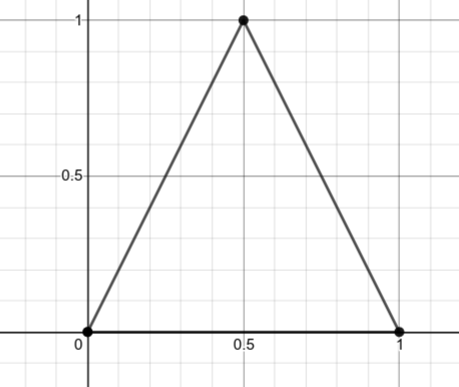
\includegraphics[width=0.5\textwidth]{q5a}\par\vspace{1cm}

The sheared triangle is as follows:

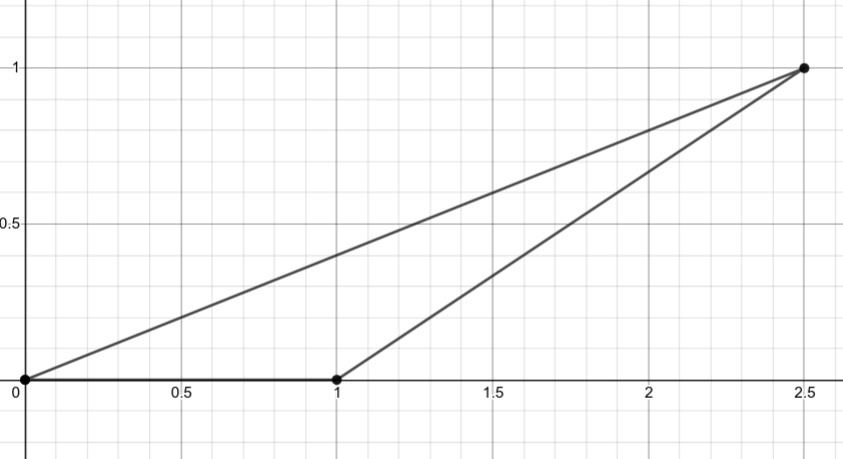
\includegraphics[width=0.5\textwidth]{q5b}\par\vspace{1cm}
\end{enumerate}
\end{enumerate}
\end{document}